\section{Project introduction}

\begin{frame}
    \frametitle{Machine Learning Pipeline}
    \tikz{
            \node[circle,fill=Button1,inner sep=3pt] (c) at (0,0){};
            \node[circle,fill=Button2,inner sep=3pt] (c) at (0.5,0){};
            \node[circle,fill=Button3,inner sep=3pt] (c) at (1,0){};
        }~~~~~~\textcolor{gold}{Figure: }High-level machine learning pipeline
    \begin{figure}[h]
        
        \centering
        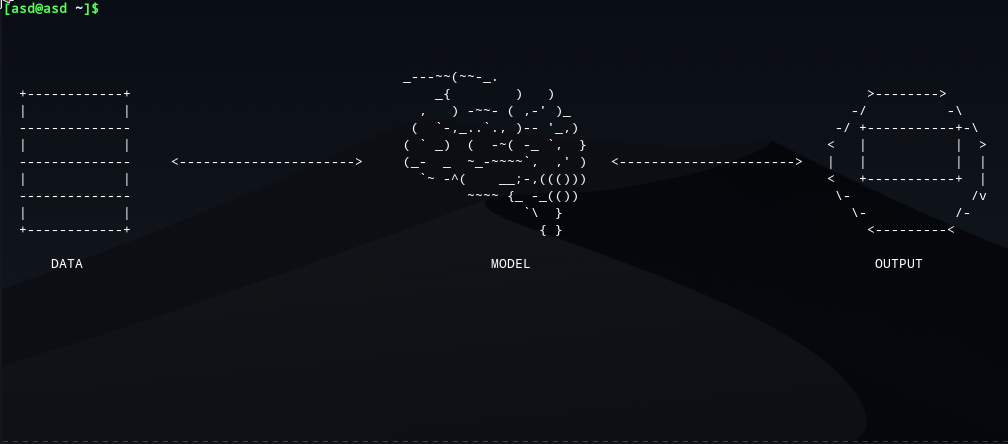
\includegraphics[scale=0.45]{ml_pipeline.png}
    \end{figure}
\end{frame}



\begin{frame}{Anomaly detection using privacy-preserving, synthetic time series data}
    
    \begin{itemize}
        \item<1-> Problem
        \begin{itemize}
            \item<1-> ML models are very \alert{data hungry}.
            \item<1-> In many cases sharing data comes with \alert{privacy risks}.
        \end{itemize}
        \item<2-> Solution:
        \begin{itemize}
            \item<2-> Promising solution: \alert{synthetic data} with privacy guarantees!
            \item<2-> Synthetic data with \alert{differential private} (DP) guarantees is a promising solution to ensure privacy independent of downstream task.
        \end{itemize}
        \item<3-> BUT:
        \begin{itemize}
            \item<3-> \alert{Privacy-Utility-Tradeoff}: Commonly, a gain in privacy results in a loss of utility. 
            \item<3-> For \alert{anomaly detection} this might not be the case (?).
        \end{itemize}
    \end{itemize}
    \onslide<4>{Goal: generate useful and privacy-preserving ECG data for anomaly detection (heartbeat arrhythmia).}
\end{frame}


\begin{frame}{Structure}
    
    \begin{figure}[h]
        \begin{flushleft}
            \tikz{
            \node[circle,inner sep=3pt] (c) at (-0.5,0){};
            \node[circle,fill=Button1,inner sep=3pt] (c) at (1.0,0){};
            \node[circle,fill=Button2,inner sep=3pt] (c) at (1.5,0){};
            \node[circle,fill=Button3,inner sep=3pt] (c) at (2.0,0){};
        }~~~~~~\textcolor{gold}{Figure: }Structure of Experiment pipeline
        \end{flushleft}
        \centering
        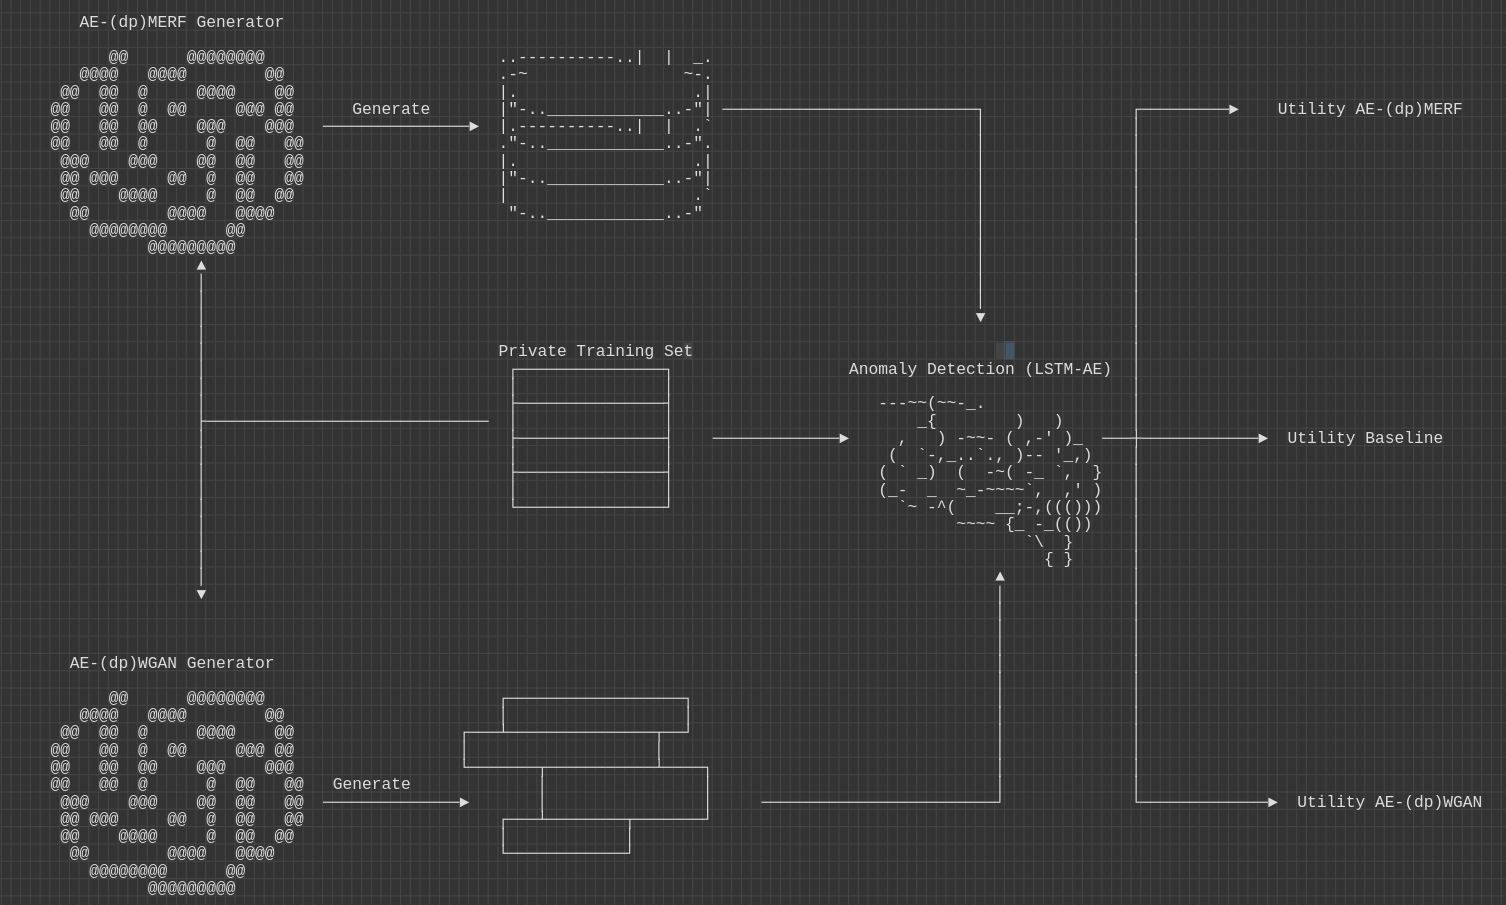
\includegraphics[scale=0.28]{str.png}
    \end{figure}
\end{frame}

\begin{frame}{Structure}
    \begin{enumerate}
        \item<1-> Train \alert{baseline model} for anomaly detection only on \alert{regular, private heartbeat data} using an LSTM-Autoencoder.
        \item<2->  \alert{Generate regular heartbeat} data using two approaches:
        \begin{itemize}
            \item<2-> [--] AE-(dp)MERF
            \item<2-> [--] AE-(dp)WGAN
        \end{itemize}
        \item<3->  Train LSTM-Autoencoder for \alert{anomaly detection on synthetic data} and \alert{test on real}.
        \item<3-> Assess \alert{utility} by measuring performance for anomaly detection (Accuracy, precision, recall, F1). 
        \item<4->  \alert{Contaminate} training data with anomalous heartbeats and repeat.
    \end{enumerate}
\end{frame}


